This section first presents the implementation details chosen to evaluate MSF in this paper, and the studied use case. Then, the compilation time of MSC is evaluated before analyzing both available parallelization techniques, data and hybrid (data and task). Finally, the impact of kernels fusions is studied.
%\CP{J'ai enlev\'e la ref au mod\`ele de perf car pas trouv\'e  dans les titres de sous-section}
%performance model proposed in Section~\ref{sect:perfs}.

%-------------------------------------
\subsection{Implementation details}

The main choices to take when implementing a specialized assembly of GA concern the technologies used for data and task parallelizations, \ie implementation choices of $DDS$ and $Scheduler$ components.

For the data-parallelization, as already detailed many times throughout the paper, a third party HPC specialist is responsible for implementing $DDS$ and $Data$ using a chosen library or external language and by following the specified interfaces of these two components. To evaluate MSF, we have played the role of HPC specialists and have implemented these components using SkelGIS, a C++ embedded DSL~\cite{CPE:CPE3494} that proposes a distributed Cartesian mesh as well as user API to manipulate structures while hiding their underlying distribution.

For task parallelism, we have chosen to use OpenMP~\cite{660313} to generate the code of the $Scheduler$ component. OpenMP targets shared-memory platforms only. Although the version 4 of OpenMP has introduced explicit support for dynamic task scheduling, our implementation only requires version 3 whose fork-join model is well suited for the static scheduling introduced in Section~\ref{sect:parallelism}.
The use of dynamic schedulers, such as provided by libgomp\footnote{\url{https://gcc.gnu.org/projects/gomp/}}, StarPU~\cite{Augonnet2011}, or XKaapi~\cite{Gautier:2013:XRS:2510661.2511383}, to directly execute the DAG $\Gamma_{dep}$ is left to future work.

As a result, MSC generates a hybrid code which uses both SkelGIS and OpenMP.
It also generates the structure of $K$ components where the developer must provide local sequential implementations of the kernels using SkelGIS API.

%-------------------------------------
\subsection{Use case description}

All evaluations presented in this section are based on a real case study of the shallow-Water Equations as solved in the FullSWOF2D\footnote{\url{http://www.univ-orleans.fr/mapmo/soft/FullSWOF/}}~\cite{Ferrari2004,CPE:CPE3494} code from the MAPMO laboratory, University of Orl\'eans.
In 2013, a full SkelGIS implementation of this use case has been performed by numericians and developers of the MAPMO laboratory~\cite{CPE:CPE3494,cordier2013fullswof,coullon:hal-00832660}. From this implementation we have kept the code of computation kernels to directly use it into $K$ components. Compared to a full SkelGIS implementation, where synchronizations and fusions are handled manually, MSF automatically compute where synchronizations are needed and how to perform a fusion without errors. To evaluate MSF on this use case we have described the FullSWOF2D simulation by using MSL. FullSWOF2D contains 3~mesh entities, 7~computation domains, 48~data and 98~computations (32~stencil kernels and 66~local kernels). Performances of the obtained implementation are compared to the plain SkelGIS implementation to show that no overheads are introduced by MSF by using \llc.

%-------------------------------------
\subsection{Multi-Stencil Compiler evaluation}

Table~\ref{fig:exectime} illustrates the execution time of each step of MSC for the FullSWOF2D example.
This has been computed on a laptop with a dual-core Intel Core i5 1.4~GHz, and 8~GB of DDR3.
MSC has been implemented in Python 2.
%
While the overall time of 4.6 seconds remains reasonable for a real case study, one can notice that the computation of the $TSP$ tree is by far the longest step.
As a matter of fact, the complexity of the algorithm for N-shapes removal is $O(n^3)$.
If this complexity is not a problem at the moment and onto this use case it could become one for just-in-time compilation or more complex simulations. The replacement of the static scheduling by a dynamic scheduling using dedicated tools (such as OpenMP 4, StarPU etc.) should solve this in the future.

\begin{table}[!h]
 \begin{center}
 \begin{tabular}{|c|c|c|c|c|}
   Step & Parser & $\Gamma_{sync}$ & $\Gamma_{dep}$ & $TSP$\\
   \hline
   Time (ms) & 1 & 2 & 4.2 & 3998.5\\
   \% & 0.022 & 0.043 & 0.09 & 86.6\\
 \end{tabular}
\caption{Execution times of the MSL compiler}
\label{fig:exectime}
 \end{center}
\end{table}

%-------------------------------------
\subsection{Data parallelism evaluation}

In this part, we disable task-parallelism to focus on data-parallelism. Two versions of the code are compared in this section: first a plain SkelGIS implementation of FullSWOF2D, where synchronizations and fusions are handled manually; second, a MSF over SkelGIS version where  synchronizations and fusions are automatically handled. SkelGIS has already been evaluated in comparison with a native MPI implementation for the FullSWOF2D example~\cite{CPE:CPE3494}. For this reason, this section uses the plain SkelGIS implementation as the reference version. This enables to evaluate both the choices made by MSC as well as the potential overheads of using \llc~\cite{l2c} that is not used in the plain SkelGIS version. The evaluations have been performed on the Curie supercomputer (TGCC, France) described in Table~\ref{tab:TGCC}. Each evaluation has been performed nine times and the median is presented in results.

\begin{table}[!ht]
\begin{center}
 \begin{tabular}{|c|c|}
     & TGCC Curie Thin Nodes\\
     \hline         
    Processor & 2$\times$SandyBridge\\
    & (2.7 GHz)\\
    Cores/node & 16 \\
    RAM/node & 64 GB\\
    RAM/core & 4GB\\
    \#Nodes & 5040 \\
    Compiler [-O3] & gcc 4.9.1\\
    MPI & Bullxmpi\\
 \end{tabular}
 \caption{\label{tab:TGCC}Hardware configuration of TGCC Curie Thin nodes.}
 \end{center}
\end{table}

\paragraph{\textbf{Weak scaling}}
Figures~\ref{fig:weak1}, \ref{fig:weak2} and~\ref{fig:weak3} respectively show weak scaling experiments tha twe have conducted. Four computation domains are evaluated: $400 \times 400$ cells by core, $600 \times 600$ cells by core and $800 \times 800$ cells by core, from 16 to 16,384 cores, as summarized in Table~\ref{tab:weak}.

\begin{table}[!ht]
\begin{center}
 \begin{tabular}{|c|c|}
    Domain size per core & Number of iterations\\
    \hline
     $400 \times 400$ & $200$\\
     $600 \times 600$ & $200$\\
     $800 \times 800$ & $200$\\
 \end{tabular}
 \caption{\label{tab:weak}Weak scaling experiments of Fig.~\ref{fig:weak1}, Fig.~\ref{fig:weak2} and Fig.~\ref{fig:weak3}.}
 \end{center}
\end{table}

\begin{figure}[t]
\begin{minipage}{.475\textwidth}
  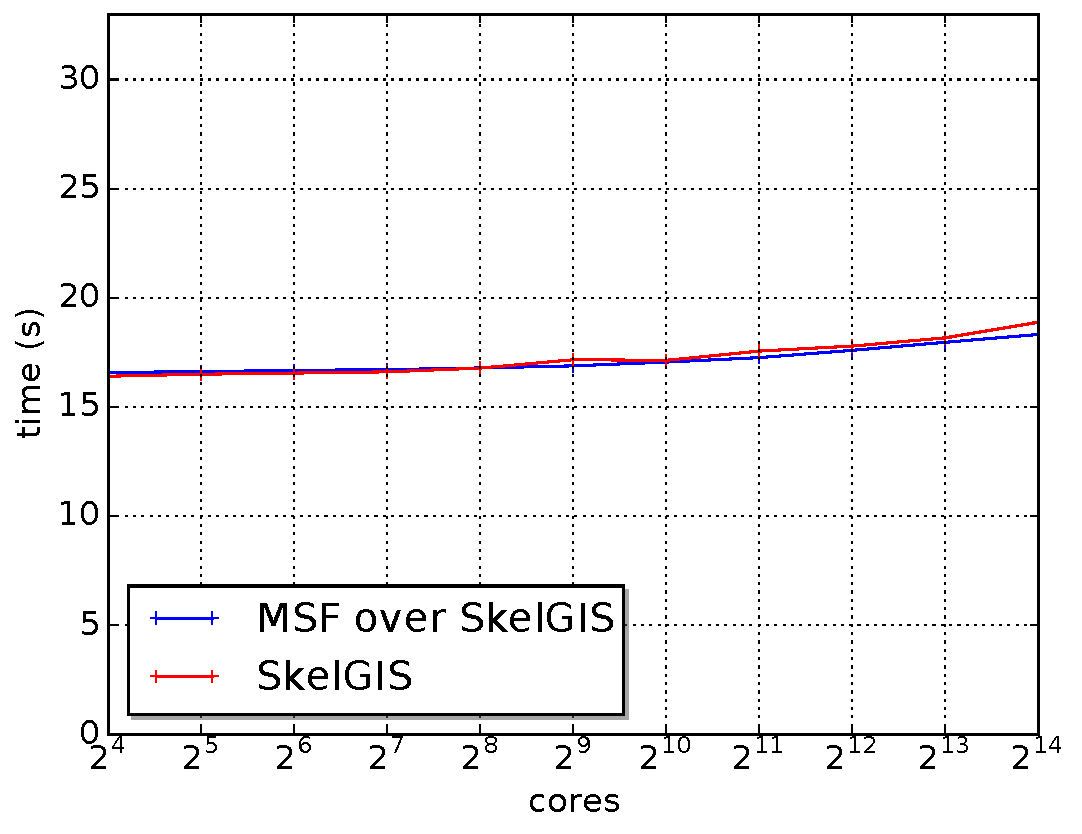
\includegraphics[width=\textwidth]{../results/weak_scaling/400_200/median_weak.pdf}
  \caption{weak-scaling with $400 \times 400$ domain per core and $200$ time iterations.}
  \label{fig:weak1}
\end{minipage}
\hfill
\begin{minipage}{.475\textwidth}
  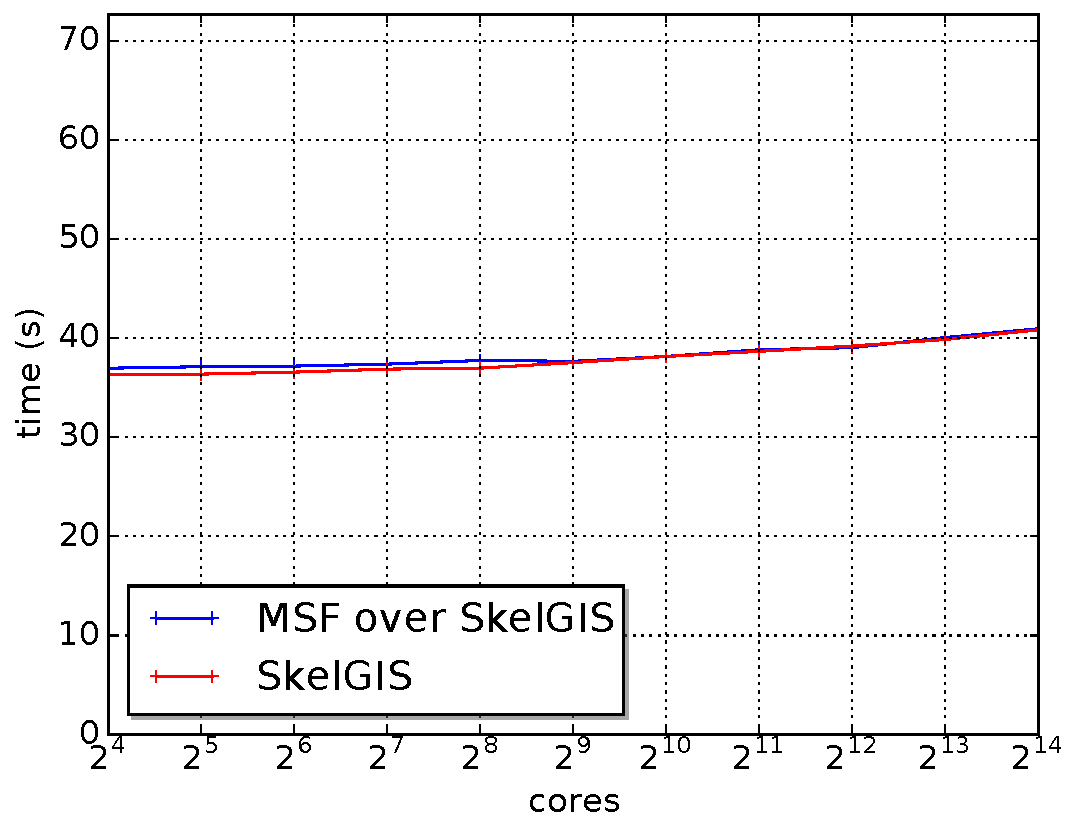
\includegraphics[width=\textwidth]{../results/weak_scaling/600_200/median_weak.pdf}
  \caption{weak-scaling with $600 \times 600$ domain per core and $200$ time iterations.}
  \label{fig:weak2}
\end{minipage}\end{figure}

\begin{figure}[t]
\begin{center}
  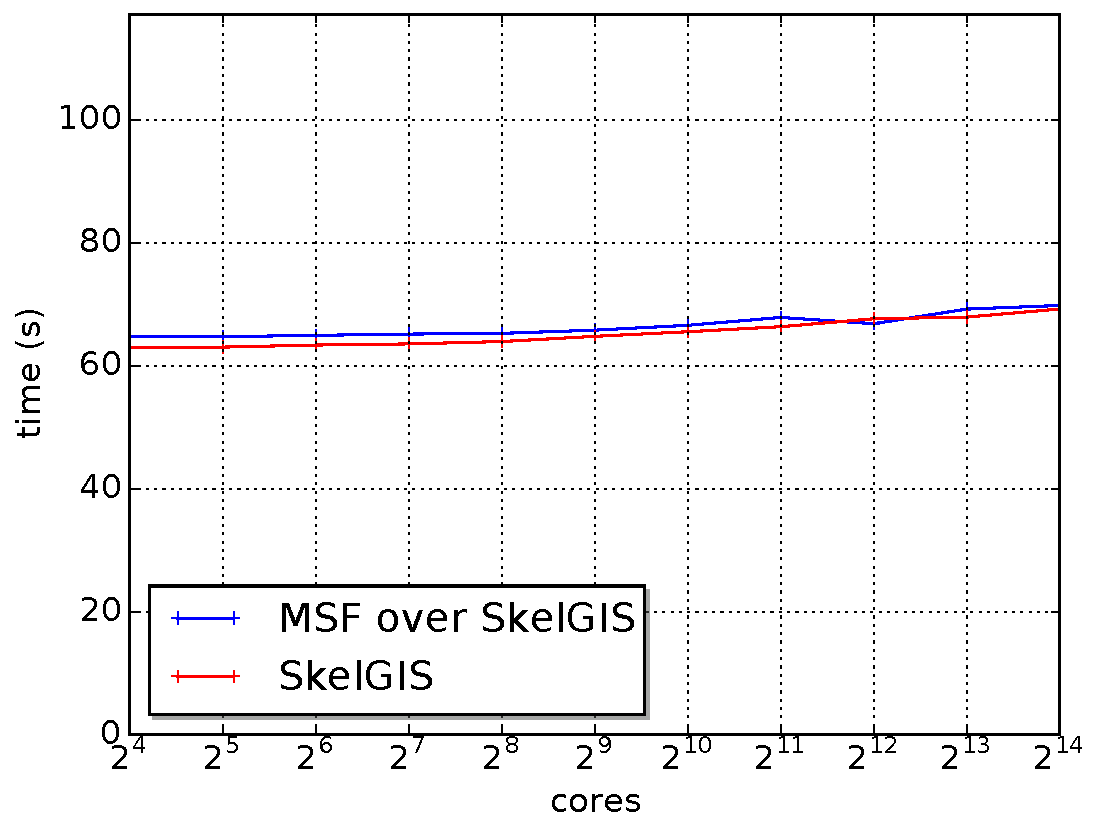
\includegraphics[width=.6\textwidth]{../results/weak_scaling/800_200/median_weak.pdf}
  \caption{weak-scaling with $800 \times 800$ domain per core and $200$ time iterations.}
  \label{fig:weak3}
 \end{center}
\end{figure}

From these results, one can notice, first, that performances of MSF are very close to the reference version using plain SkelGIS. This is a very good result which shows first that MSC performs good synchronizations and fusions, and second that overheads introduced by \llc are limited thanks to a good component granularity in the Generic Assembly.

However, it seems that a slightly drop of performance happens when the domain size per core increases. This performance decrease is really small though, with a maximum difference between the two versions of 2.83\% in Fig.~\ref{fig:weak3}.
%\CP{Quelle figure? est ce \ref{fig:weak3} pour de petit nombre de core? Si oui, \`a mod\'erer car MSF devient meilleur quand le nombre de core augmente}

The only noticeable difference between the two versions are due to \llc which load dynamic libraries at runtime. Because of this particularity, components of \llc are compiled with the \emph{-fpic} compilation flag\footnote{\llc has been recently extended with the possibility of static linking.} while the SkelGIS version does not. This flag can have slight positive or negative effects on code performance depending on the situation and might be responsible for the observed difference.

%\HC{another benchmark to show that with the static version of \llc the problem disappear ?}

\paragraph{\textbf{Strong scaling}}
\begin{figure}[t]\begin{center}
  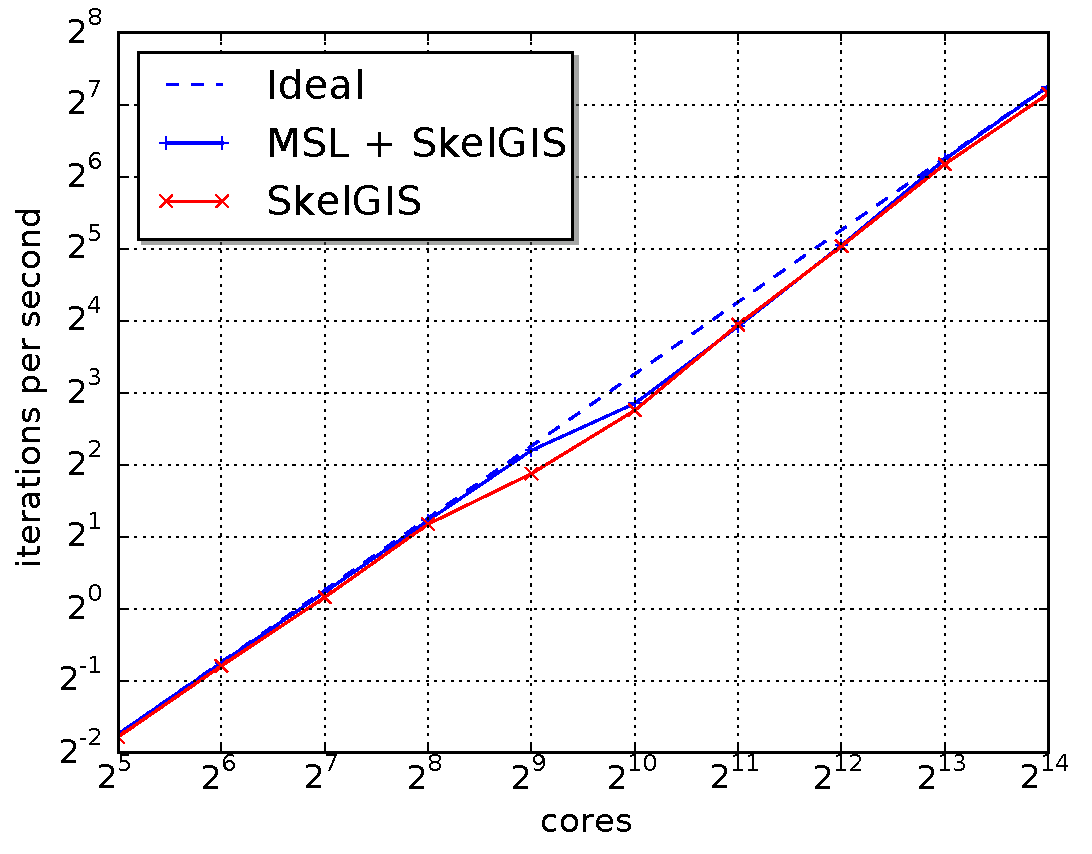
\includegraphics[width=.6\textwidth]{../results/strong_scaling/10K_1K/median_strong.pdf}
  \caption{Strong scaling on a $10k \times 10k$ domain and $1000$ time iterations.}
  \label{fig:strong}
\end{center}\end{figure}

Figure~\ref{fig:strong} shows the number of iteration per second for a 10k$\times$10k global domain size from 16 to 16,384 cores. The total number of time iterations for this benchmark is $1000$. In addition to the reference SkelGIS version, the ideal strong scaling is also plotted in the figure.

First, one can notice that the strong scaling evaluated for the MSF version is close to the ideal speedup up to 16,384 cores, which is a very good result. Moreover, no overheads are introduced by MSF which shows that automatic synchronizations and automatic fusions enable the same level of performance than the one manually written into the plain SkelGIS version. Finally, no overheads are introduced by components of \llc. A small behavior difference can be noticed with $2^9=512$ cores, however this variation is no longer observed with 1024 cores. %We have not analyzed this behavior that we consider not fundamental.
%\CP{Un commentaire sur le decrochage par rapport au perfect speedup pour $2^9--2^{12}$??}

%\paragraph{\textbf{Fusion}} Finally, we evaluate loop fusions automatically proposed by MSF from the $TSP$ tree of computation kernels. Figure~\ref{fig:fusion} shows the number of iterations per second as a function of the number of cores with and without fusions. This benchmark is performed on FullSWOF2D onto a $500 \times 500$ domain size with $200$ time iterations. As explained in Section~\ref{sect:fusion}, the MSF loop fusion happens at a high level and is most of the time done naturally by a computer scientist. However, for a non computer scientist which write its numerical codes, an automatic proposition of such fusions avoid errors, particularly for a parallel execution. Moreover, one can notice that the performance is clearly improved (around 40\%) by this fusion.
%
%\begin{figure}[!h]\begin{center}
%  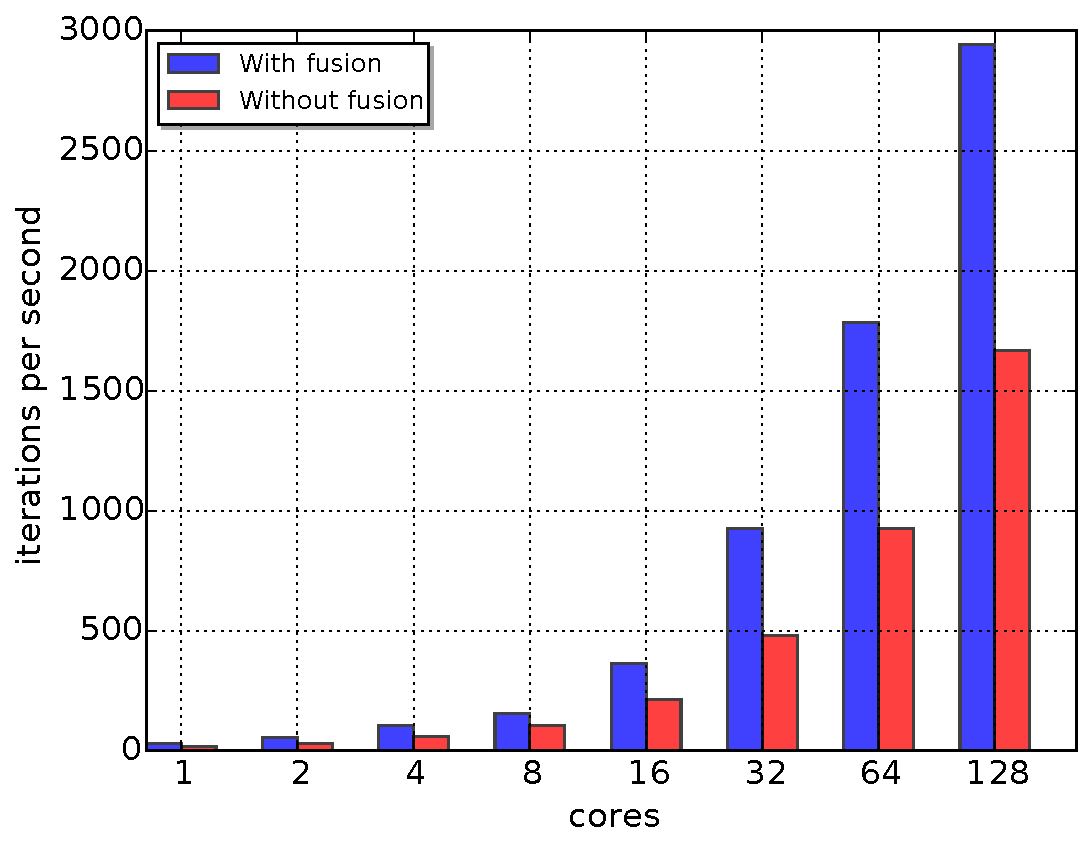
\includegraphics[width=.6\textwidth]{../results/task_scaling/500_200/fusVSbase.pdf}
%  \caption{Strong scaling on a 500x500 domain size with $200$ time iterations, with and without fusions proposed by MSF.}
%  \label{fig:fusion}
%\end{center}\end{figure}
%
%\HC{another benchmark with and without fusion fro task parallelization ?}

%-------------------------------------
\subsection{Hybrid parallelism evaluation}

In this section, we add task parallelism to evaluate the hybrid parallelization offered by MSF. The MSF implementation evaluated in this paper relies on SkelGIS and OpenMP.

The series-parallel tree decomposition $TSP$ of this simulation, extracted by MSC, is composed of 17 nodes labeled as sequence $\mathcal{S}$ and 18 nodes labeled as parallel $\mathcal{P}$. 

We define the \emph{level of parallelism} as the number of parallel tasks inside one fork of the fork/join model. The fork/join model obtained for FullSWOF2D is composed of 18 fork phases (corresponding to $\mathcal{P}$ nodes of $TSP$). Table~\ref{fig:freq} represents the number of time (denoted frequency) a given level of parallelism is obtained inside fork phases.

\begin{table}[th]
 \begin{center}
 \begin{tabular}{|c|c|c|c|c|c|c|c|c|}
   Level & 1 & 2 & 3 & 4 & 6 & 10 & 12 & 16\\
   \hline
   Frequency & 2 & 1 & 3 & 5 & 3 & 1 & 1 & 2\\
 \end{tabular}
\caption{Parallelism level and the number of times this parallelism level appears into fork phases.}
\label{fig:freq}
 \end{center}
\end{table}

One can notice that the level of task parallelism extracted from the Shallow water equations is limited by two sequential parts in the application (level 1). Moreover, a level of 16~parallel tasks is reached two times, and five times for the fourth level.
This means that if two cores are dedicated to task parallelism, the two sequential parts of the code will not take advantage of these two cores, and that no part of the code would benefit from more than 16 cores. The task parallelism, as proposed in this paper (\ie where each kernel is a task) is therefore insufficient to take advantage of a single node of modern clusters that typically supports more than 16 cores.

\begin{figure}[th]\begin{center}
  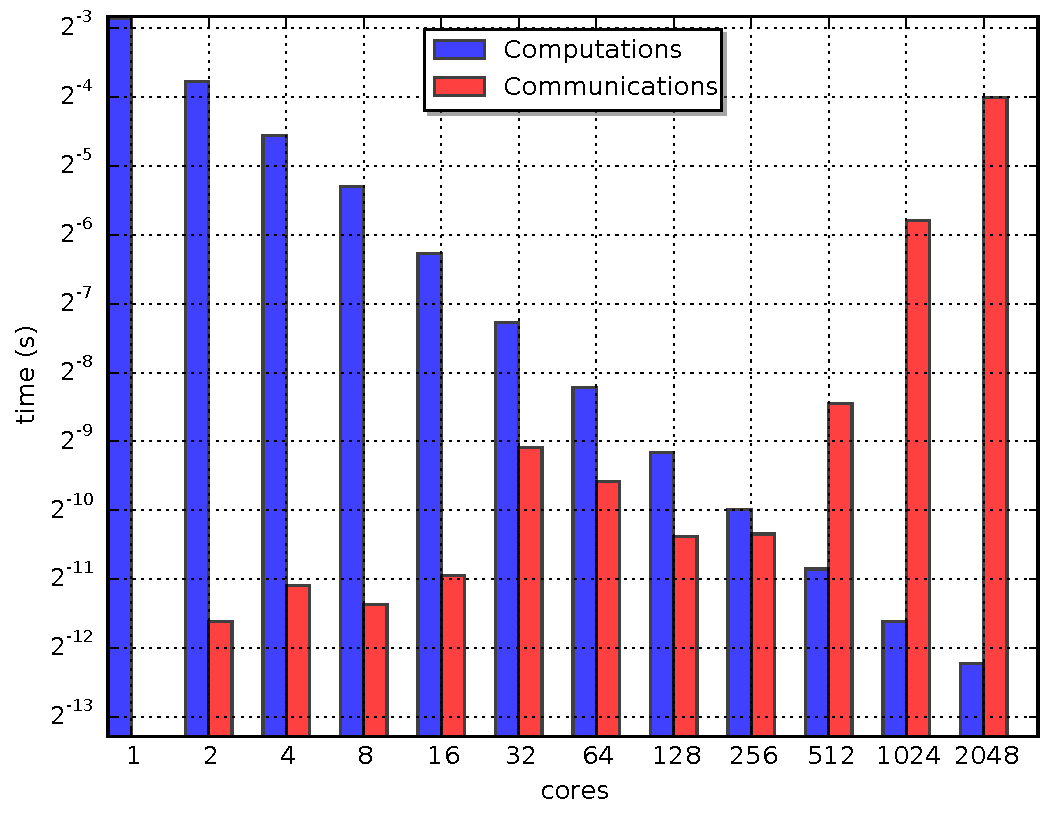
\includegraphics[width=.6\textwidth]{../results/task_scaling/500_200/analytic/times.pdf}
  \caption{Computation vs communication times for a single time iteration using the data parallelization technique.}
  \label{fig:limit}
  %\CP{es tu sûr que le temps soit en puissance de 2 et pas en puissance de 10? C'est strange.}
\end{center}\end{figure}

On the other hand, Figure~\ref{fig:limit} illustrates limitations of data parallelization technique alone. This figure displays the execution time (with a logarithmic scale) of FullSWOF2D while increasing the number of cores for a fix domain size of $500 \times 500$ with a total of $200$ time iterations (\ie this is a strong scaling). One can note that times are really small. Actually the time represented in Fig.~\ref{fig:limit} is the time spent into a single time iteration. The speedup of this same benchmark is represented in blue in Figure~\ref{fig:close}. One can note that the scaling is not as good as the one presented in Figure~\ref{fig:strong}. 
The main difference between these two benchmarks is the domain size. In the benchmark of Figure~\ref{fig:strong} the domain size is $10k \times 10k$ which means that using $2^8 = 256$ cores, for example, each core has to compute only a $625 \times 625$ sub-domain. On the other hand, using $2^8$ cores in Figure~\ref{fig:close} each core has to compute a $31 \times 31$ sub-domain. Figure~\ref{fig:limit} shows why the speedup is not as good as the one with a bigger domain size.  

Actually, in this figure, while the computation time (in blue) decreases linearly with the number of core used, the communication behavior (in red) is much more erratic. Between 2 and 16 cores, communications are performed inside a single node thus the time is small and nearly constant. There is a small oscillation that might be explained by the partitioning differences. SkelGIS performs a two dimensional partitioning strategy. For this reason a smaller number of bytes are communicated using 2 cores than using 4, and using 8 cores than using 16 cores. Starting from 32 cores, each node is fully used and more than one node is used. From this point thus the communication time is typically modeled as $L+S/B$ where $L$ is the latency, $S$ the data size and $B$ the bandwidth. This explains the decrease of communication time from 32 to 128 cores where the data sizes communicated by each process decreases. The increases observed after $128$ cores might be due to the fact that with the increased number of processes the fat-tree becomes deeper and the latencies increase.

\begin{figure}[th]\begin{center}
  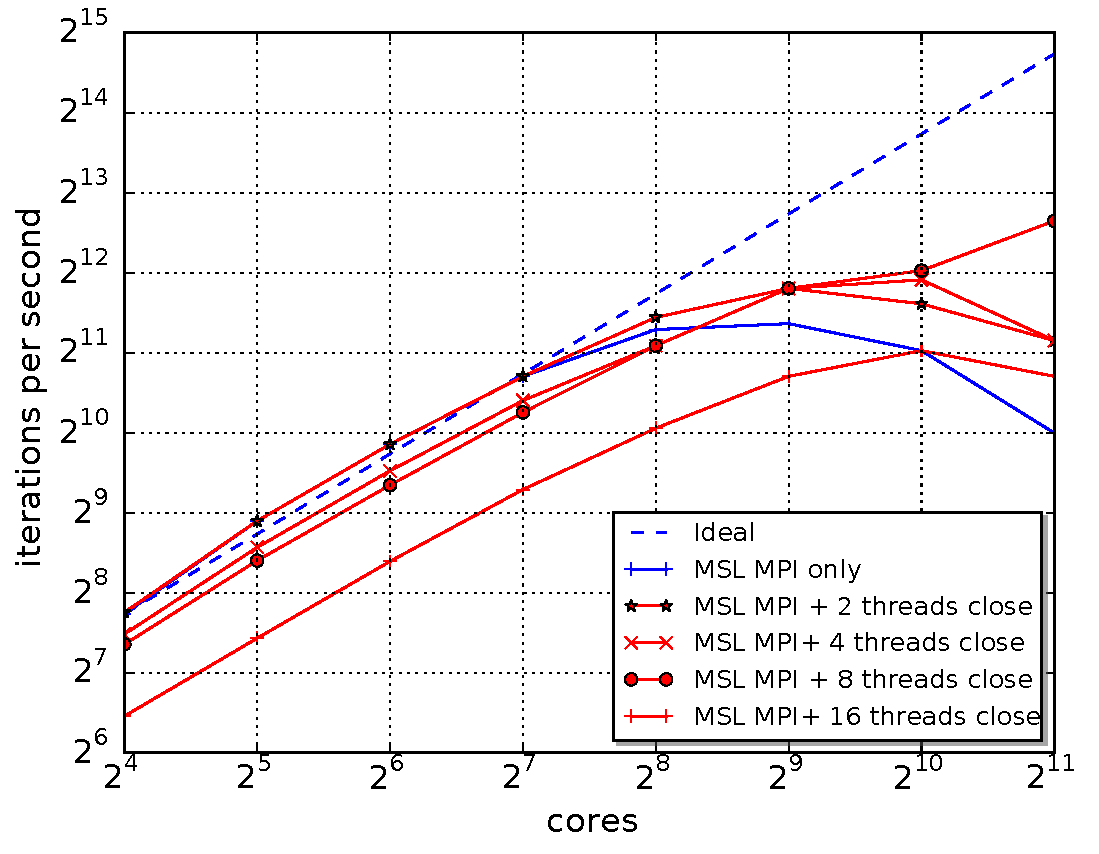
\includegraphics[width=.6\textwidth]{../results/task_scaling/500_200/base_close_median.pdf}
  \caption{Strong scaling comparisons between data parallelization and hybrid parallelization. A \emph{close} OpenMP clause is used to bind threads onto cores.}
  \label{fig:close}
\end{center}\end{figure}

All in all, when the number of core increases, the computation/communication ratio becomes poorer and poorer. As a result, the data parallelism alone fails to provide enough parallelism to leverage the whole machine and other sources of parallelism have to be found. As expected, in  Figure~\ref{fig:close} the speedup bends down from 256 to 2048 cores. The same problem would happened in previous experiment of Figure~\ref{fig:strong}, however as the domain size is larger, the phenomena appears with more cores. 

As task parallelism fails to scale from 16 cores, and as data parallelism also fails to scale when the communication cost overpass the execution time, an hybrid parallelization strategy is proposed by MSF and is evaluated below.

In addition to the blue curve, Figure~\ref{fig:close} shows speedups for the same example ($500 \times 500$ domain with $200$ iterations) but using an hybrid parallelization. Figure~\ref{fig:close} shows a comparison with 2, 4, 8 and 16 cores per MPI process for task parallelization.

For example, the purple curve shows the parallelization which uses for each data parallelization process (\ie MPI process) 8 additional cores for task parallelization. As a result, for example, when using 2 machines of the TGCC cluster, with a total of 32 cores, 4 cores are used for SkelGIS MPI processes, for data parallelization, and for each one 8 cores are used for task parallelization ($4 \times 8 = 32$). This respects $P = P_{data} \times P_{task}$ as presented in Section~\ref{sect:perfs}.
As a result, and as explained in Section~\ref{sect:perfs}, quantities that are responsible for communications are less divided into sub-domains. Therefore, the effect observed with the blue curve is delayed to a higher number of cores.

From 2 to 8 cores, the improvement of the strong scaling is clear. However, reaching 16 cores, an important initial overhead appears and in addition to this, the curve bends down rapidly instead of improving the one with 8 cores for task parallelization. Two different phenomena happen in this case.

First, thin nodes of the TGCC Curie are built with two NUMA socket each of 8 cores. As a result, when increasing the number of OpenMP cores for task parallelization from 8 to 16 cores, an overhead is introduced by exchanges of data between memories of the two NUMA sockets. This phenomena is illustrated in Figure~\ref{fig:spread}. In this figure, a different binding strategy is used. A binding strategy is the way the scheduler binds threads onto available cores. The strategy used in Figure~\ref{fig:spread} is called \emph{spread} (instead of \emph{close} in Figure~\ref{fig:close}). This strategy binds threads on cores in order to spread as much as possible onto resources, which means that the two NUMA sockets are used whatever the number of cores used for tasks is. As a result, and as shown in the figure, using 2, 4 and 8 cores an initial overhead is introduced as the one observed in Figure~\ref{fig:close}. This shows that the initial overhead with 16 cores is due to NUMA effects.

\begin{figure}[!h]\begin{center}
  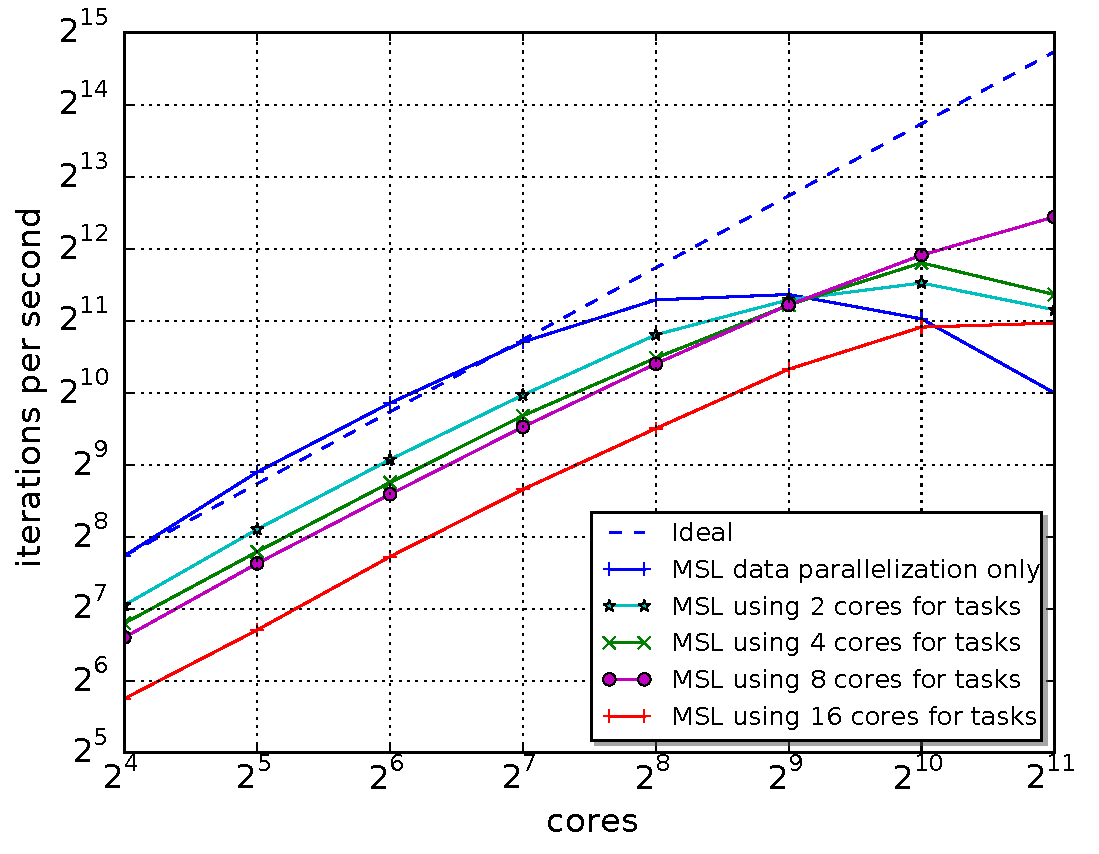
\includegraphics[width=.6\textwidth]{../results/task_scaling/500_200/base_spread_median.pdf}
  \caption{Strong scaling comparisons between data parallelization and hybrid parallelization. A \emph{spread} OpenMP clause is used to bind threads onto cores.}
  \label{fig:spread}
\end{center}\end{figure}

The second phenomena that happens in Figure~\ref{fig:close} using 16 cores is due to the level of parallelism introduced by the task parallelization technique. Actually, as illustrated in Table~\ref{fig:freq}, only two forks of $TSP$ can take advantage of 16 cores among a total of 18 forks. This phenomena has been mentioned in Section~\ref{sect:perfs} by the variable $F_{task}$ and the fact that it is not always true that $F_{task}=P_{task}$. This explains why using 16 cores is less efficient than using 8 cores, even when the two NUMA sockets are always used as in Figure~\ref{fig:spread}.

Finally, to validate the performance model introduced in Section~\ref{sect:perfs}, and to understand when the hybrid parallelization becomes more interesting than the data parallelization, Figure~\ref{fig:tth2} represents $T_{COM1}$ and $T_{COM2}+T_{task}$ of Equation~(\ref{eq:hyb}), for the best case, \ie when 8 cores are used in Figure~\ref{fig:close}.  Figure~\ref{fig:tth2} and Table~\ref{fig:tth} presents results of these measurements. Results perfectly matches Figure~\ref{fig:close} for 8 cores per MPI process. As a result, the hybrid parallelization is better for 512 cores or more in this case.

\begin{table}[!h]
 \begin{center}
 \begin{tabular}{|c|c|c|c|c|}
    \hline 
    & $T_{COM1}$ & $T_{COM2}$ & $T_{task}$ & Equation~(\ref{eq:hyb})\\
   \hline
   16 cores ($2 \times 8$) & 0.0005 & 0.00032 & 0.013 & False\\
   32 cores ($4 \times 8$) & 0.0018 & 0.00045 & 0.0062 & False\\
   64 cores ($8 \times 8$) & 0.0013 & 0.00038 & 0.0034 & False\\
   128 cores ($16 \times 8$) & 0.00075 & 0.0005 & 0.0023 & False\\
   256 cores ($32 \times 8$) & 0.00077 & 0.0018 & 0.001 & False\\
   512 cores ($64 \times 8$) & 0.0029 & 0.0013 & 0.00052 & True\\
   1024 cores ($128 \times 8$) & 0.018 & 0.00075 & 0.00029 & True\\
   2048 cores ($256 \times 8$) & 0.0623 & 0.00077 & 0.00016 & True\\
   \hline
 \end{tabular}
\caption{Execution times (seconds) of $T_{COM1}$, $T_{COM2}$ and $T_{task}$ for 8 cores for task parallelization. Verification of the Equation~(\ref{eq:hyb}).}
\label{fig:tth}
 \end{center}
\end{table}

\begin{figure}[!h]\begin{center}
  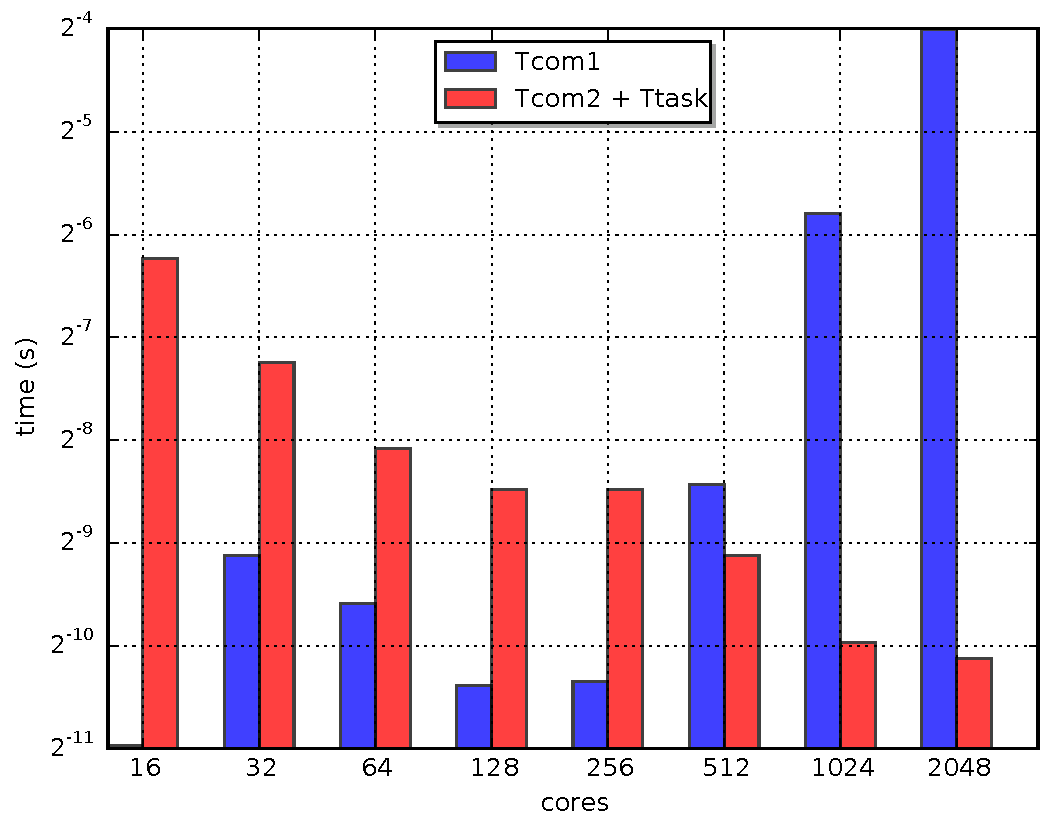
\includegraphics[width=.6\textwidth]{../results/task_scaling/500_200/analytic/tth.pdf}
  \caption{Execution times (seconds) for a single time iteration of $T_{COM1}$ and $T_{COM2} + T_{task}$ for 8 cores for task parallelization. Verification of the Equation~(\ref{eq:hyb}).}
  \label{fig:tth2}
%\CP{Time en puissance de 2 ou de 10 ?}
\end{center}\end{figure}

%-------------------------------------------------
\subsection{Fusion evaluation}
\label{sect:fus}
%-------------------------------------------------

In this section we propose an evaluation of the fusion optimization. From the $TSP$ tree computed by MSC it is possible, according to specific conditions, to merge domain loops of kernels, thus optimizing the use of cache memories. This optimization is called a fusion and has been introduced in Section\ref{sect:fusion}. Three fusion optimizations
%\CP{les rappeler !}
%
have been formally detailed in Section~\ref{sect:fusion}. The two first one of Figures~\ref{fig:fus1} and~\ref{fig:fus2} have been automatically detected by MSF in our case study (\ie scatter optimization has not been detected).

Figure~\ref{fig:fusion} shows the number of iterations per second as a function of the number of cores with and without fusions. This benchmark is performed on FullSWOF2D onto a $500 \times 500$ domain size with $200$ time iterations, and by using data parallelism alone (without tasks). As explained in Section~\ref{sect:fusion}, the MSF loop fusion happens at a high level. Most of the time such fusions are done naturally by a computer scientist. However, an automatic detection of such fusions avoids errors, particularly for a parallel execution. In addition to this, more advanced fusion cases, such as a scatter are more difficult to deduce. In FullSWOF2D a total of  62 fusions are proposed by MSF over a total of 98 computation kernels. Figure~\ref{fig:fusion} shows that the performance is clearly improved (around 40\%) by these fusions.

\begin{figure}[!h]\begin{center}
  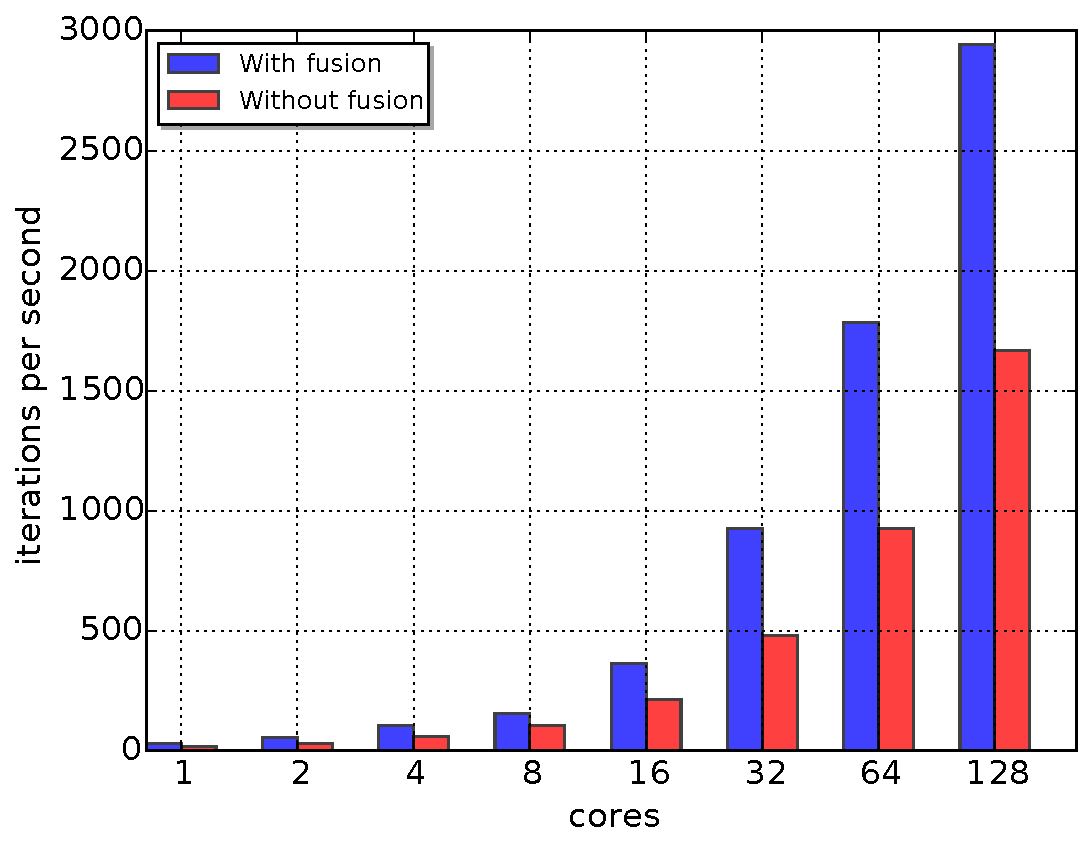
\includegraphics[width=.6\textwidth]{../results/task_scaling/500_200/fusVSbase.pdf}
  \caption{Strong scaling on a 500x500 domain size with $200$ time iterations, with and without fusions proposed by MSF.}
  \label{fig:fusion}
\end{center}\end{figure}

However, fusion optimizations are not always relevant. To illustrate this, we are using the same benchmark of FullSWOF2D onto a $500 \times 500$ domain size with $200$ time iterations, however we compare data parallelism and hybrid parallelism both with and without fusion. 

Blue curves of Figure~\ref{fig:fusion1} represent results for data parallelism with and without fusion. One can note that the best performance, as expected, is reached by the version using fusions. Red curves represent results by using 2 cores per MPI process dedicated to tasks, with and without fusion again. One can note that the best performance is also reached by the version using fusion.
%\CP{PARAGRAPHE A ADAPTER SUIVANT LES MODIFS DE LA FIGURE: 1 ou 2 exp dans la figure?}

\begin{figure}[!h]\begin{center}
  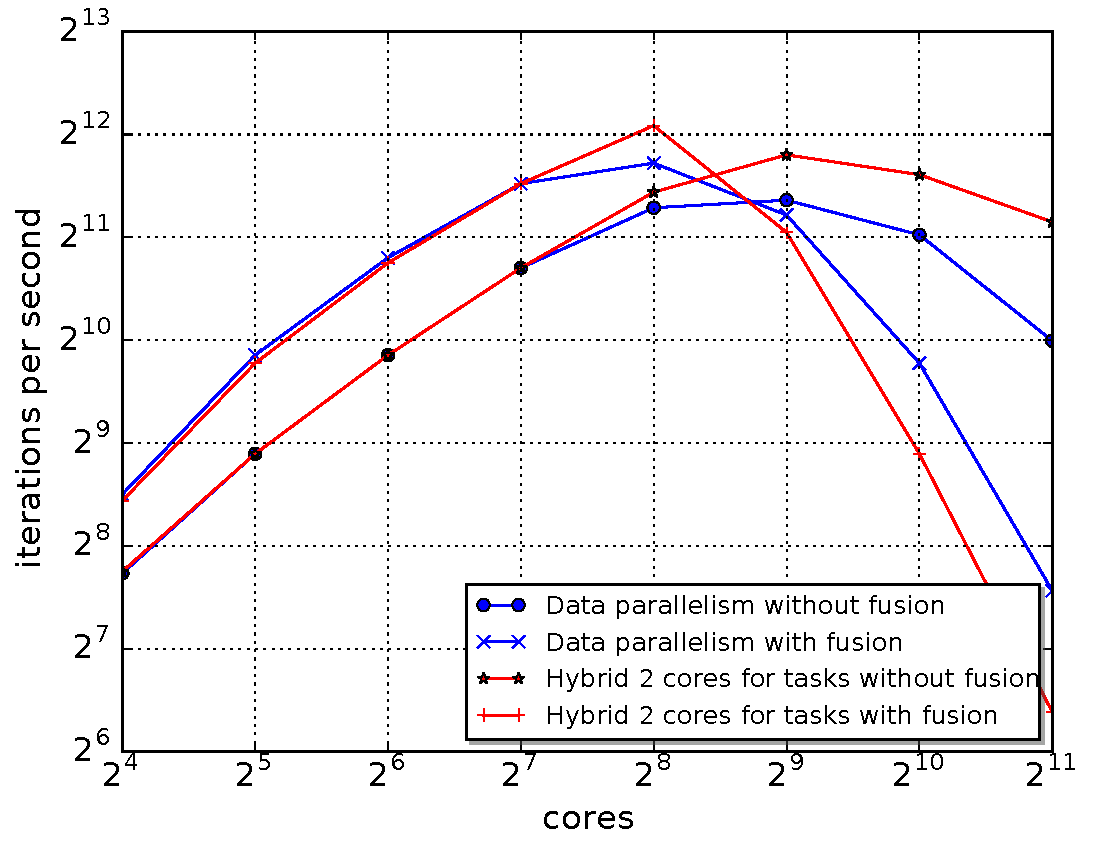
\includegraphics[width=.6\textwidth]{../results/task_scaling/500_200/withwithout2_close_median.pdf}
  \caption{String scaling on a 500x500 domain size with $200$ time iterations. Blue curves represent strong scaling for data parallelism with and without fusion. Red curves represent strong scaling by using 2 cores per MPI process dedicated to tasks, with and without fusion.}
  \label{fig:fusion1}
  %\CP{A FINIR !!! ERREUR DANS LEGENDES AUSSI. COULEUR PROCHES}
\end{center}\end{figure}

However, to deeper analyze this results, we propose a second evaluation presented in Figure~\ref{fig:fusion2}. The blue curves are exactly the same one than in Figure~\ref{fig:fusion1}. The red curves, on the other hand, represent results by using 8 cores per MPI process dedicated to tasks, with and without fusion. Interesting results appears in this figure as the hybrid version using fusions is less efficient than the one without fusions. As already explained, this result is due to the fact that fusions reduce the number of tasks from 98 to 36 resulting in a non optimized use of eight cores for task parallelism. By using only 2 cores per MPI process (in Figure~\ref{fig:fusion1}) the 36 computation kernels were enough to feed the two cores, while it is not for eight.

\begin{figure}[!h]\begin{center}
  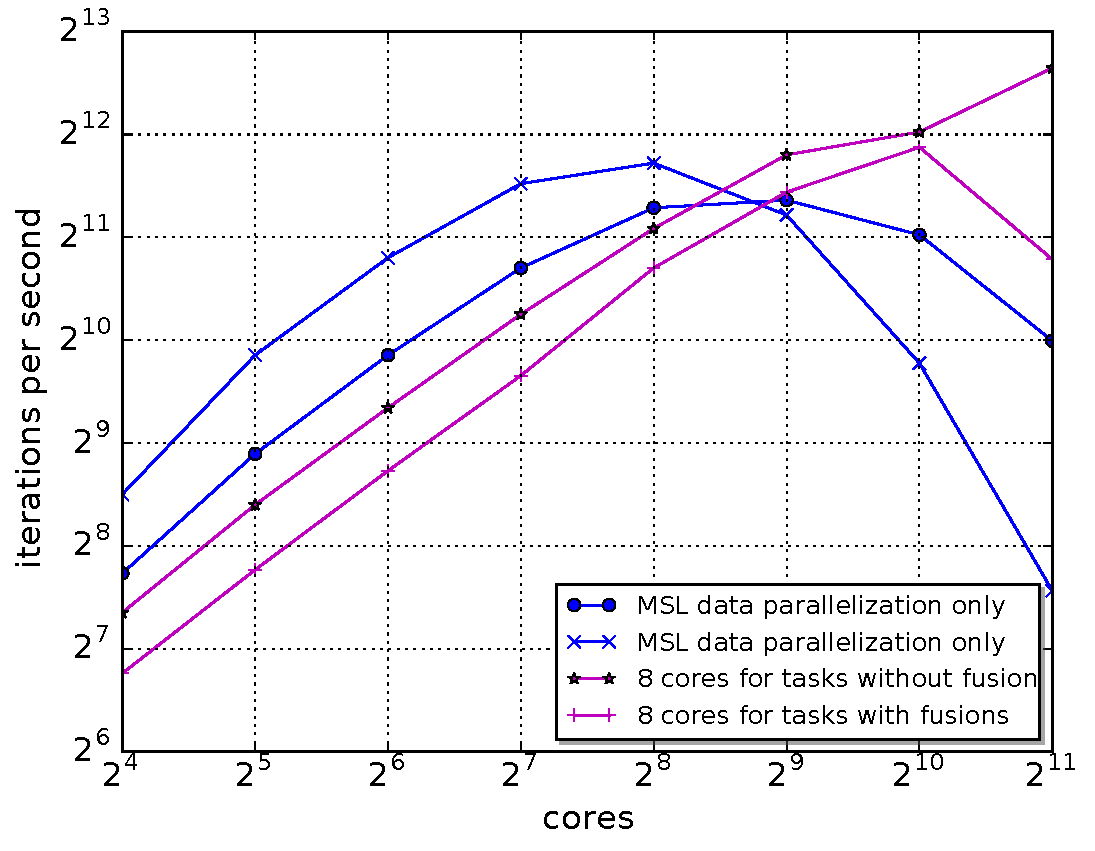
\includegraphics[width=.6\textwidth]{../results/task_scaling/500_200/withwithout8_close_median.pdf}
  \caption{String scaling on a 500x500 domain size with $200$ time iterations. Blue curves represent strong scaling for data parallelism with and without fusion, thus are exactly the same than blue curves of Fig.~\ref{fig:fusion1}. Red curves represent strong scaling by using 8 cores per MPI process dedicated to tasks, with and without fusion.}
  \label{fig:fusion2}
    %\CP{A FINIR !!! ERREUR DANS LEGENDES AUSSI.}
\end{center}\end{figure}
As a result, if fusion optimization incurs a too large reduction of the number of tasks to feed dedicated cores, the problem observed for 16 cores in Figure~\ref{fig:close} happens earlier which reduces obtained performances. For this reason, MSF performs fusions only when data parallelization is used alone. This choice could be more intelligent but this is the subject of future work.
